\documentclass{article}

\usepackage{graphicx}
\usepackage{tikz}
\usepackage{tikzsymbols}
\usetikzlibrary{calc,patterns,shapes.geometric}
\pagestyle{empty}
\usepackage[margin=0pt]{geometry}
\geometry{papersize={14in,12in}}

\def\centerarc[#1](#2)(#3:#4:#5){\draw[#1] ($(#2)+({#5*cos(#3)},{#5*sin(#3)})$) arc (#3:#4:#5);}

\begin{document}
	\begin{figure}
		\centering
		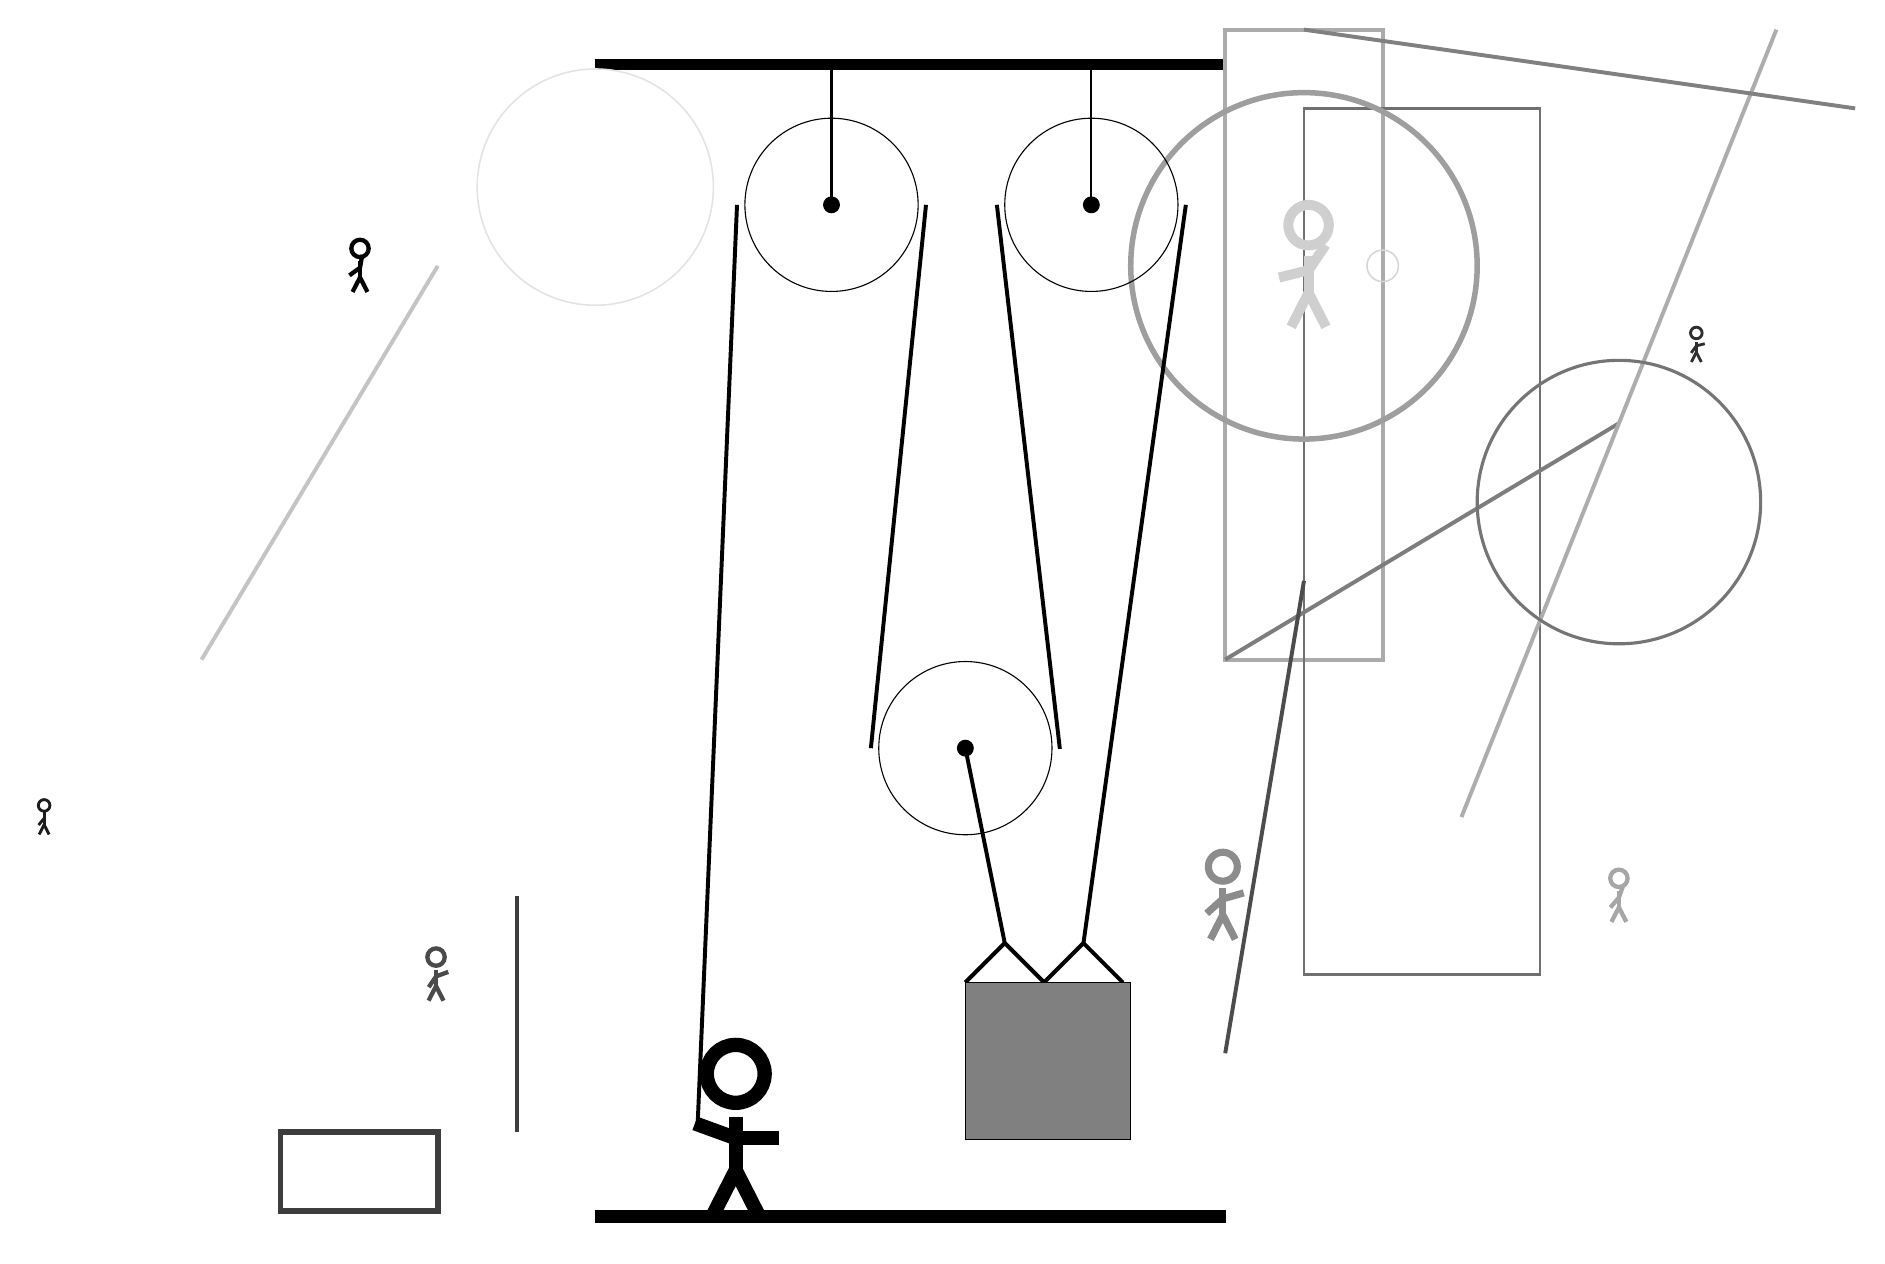
\begin{tikzpicture}
			%%%%% START %%%%%
			
			\draw[fill=black] (-2, 11.5) rectangle (6, 11.625);
			
			\draw[line width=0.5mm, color=black!33] (8, 12) rectangle (6, 4);
			
			\draw[line width=0.3mm, color=black!56] (7, 11) rectangle (10, 0);
			\draw[line width=0.5mm, color=black!51](6, 4) -- (11, 7);
			\node[line width=0.5mm, color=black!45] at (6, 1) {\Strichmaxerl[5][42][16]};
			\draw[line width=0.5mm, color=black!32](9, 2) -- (13, 12);
			\node[line width=0.6mm, color=black!99] at (-5, 9) {\Strichmaxerl[3][36][80]};
			\node[line width=0.7mm, color=black!82] at (12, 8) {\Strichmaxerl[2][54][14]};
			\node[line width=0.3mm, color=black!71] at (-4, 0) {\Strichmaxerl[3][56][20]};
			\draw[line width=0.5mm, color=black!76](-3, 1) -- (-3, -2);
			
			\node[line width=0.2mm, color=black!35] at (11, 1) {\Strichmaxerl[3][49][71]};
			
			\draw[line width=0.5mm, color=black!50](7, 12) -- (14, 11);
			
			\draw[line width=0.5mm, color=black!70](7, 5) -- (6, -1);
			\draw [line width=0.2mm, color=black!16](8, 9) circle (0.2);
			
			\draw[line width=0.2mm, color=black!99] (-3, 0) rectangle (-3, 0);
			\draw [line width=0.7mm, color=black!38](7, 9) circle (2.2);
			\draw [line width=0.2mm, color=black!11](-2, 10) circle (1.5);
			\node[line width=0.6mm, color=black!89] at (-9, 2) {\Strichmaxerl[2][51][90]};
			
			\draw[line width=0.7mm, color=black!76] (-4, -2) rectangle (-6, -3);
			\node[line width=0.4mm, color=black!19] at (7, 9) {\Strichmaxerl[7][14][56]};
			
			\draw [line width=0.4mm, color=black!54](11, 6) circle (1.8);
			\draw[line width=0.5mm, color=black!23](-7, 4) -- (-4, 9);
			
			\draw (1, 9.775) circle (1.1);
			\draw[fill=black] (1, 9.775) circle (0.1);
			\draw[thick] (1, 9.775) -- (1, 11.5);
			
			\draw (4.3, 9.775) circle (1.1);
			\draw[fill=black] (4.3, 9.775) circle (0.1);
			\draw[thick] (4.3, 9.775) -- (4.3, 11.5);
			
			\draw (2.7, 2.875) circle (1.1);
			\draw[fill=black] (2.7, 2.875) circle (0.1);
			
			\draw[line width=0.5mm]  (2.7, -0.1) -- (3.2, 0.4) -- (3.7, -0.1) -- (4.2, 0.4) -- (4.7, -0.1);
			\draw[fill=black!50] (2.7, -0.1) rectangle (4.8, -2.1);
			
			\draw[line width=0.5mm](-0.7, -1.9) -- (-0.2, 9.775);
			\centerarc[line width=0.5mm](1, 9.775)(0:180:1.2000000000000002);
			\draw[line width=0.5mm](2.2, 9.775) -- (1.5, 2.875);
			\centerarc[line width=0.5mm](2.7, 2.875)(180:370:1.2000000000000002);
			\draw[line width=0.5mm] (3.9, 2.865) -- (3.1, 9.775);
			\centerarc[line width=0.5mm](4.3, 9.775)(0:180:1.2000000000000002);
			\draw[line width=0.5mm](4.2, 0.4) -- (5.5, 9.775);
			\draw[line width=0.5mm] (3.2, 0.4) -- (2.7, 2.875);
			
			\node at (-0.2, -2) {\Strichmaxerl[10][-20][0]};
			
			\draw[fill=black] (-2, -3) rectangle (6, -3.15);
			
			%%%%% END %%%%%
		\end{tikzpicture}
	\end{figure}	
\end{document}